\section{Fundamentos F\'isicos}

\subsection{Pozos Cu\'anticos Acoplados}
\begin{frame}[t]
\frametitle{\secname}
\framesubtitle{\subsecname}
\vspace{-0.5cm}
\begin{tikzpicture}[remember picture, overlay]
\node<1->[anchor = north west, text width =0.73\textwidth, yshift = -0.75cm](txt) at (current page.north west) {
	\begin{tcolorbox}[width =\textwidth,title=\subsecname]
	\begin{itemize}
	\item<1-> Sistemas Nanoestructurados$\rightarrow$ Pozo Cu\'antico Simple.
	\item<2-> Pozos Cu\'anticos Acoplados
	\end{itemize}
	\end{tcolorbox}	
};

\node<1->[anchor=north west,inner sep=0mm,yshift=10mm,xshift=-2mm](f) at (txt.north east){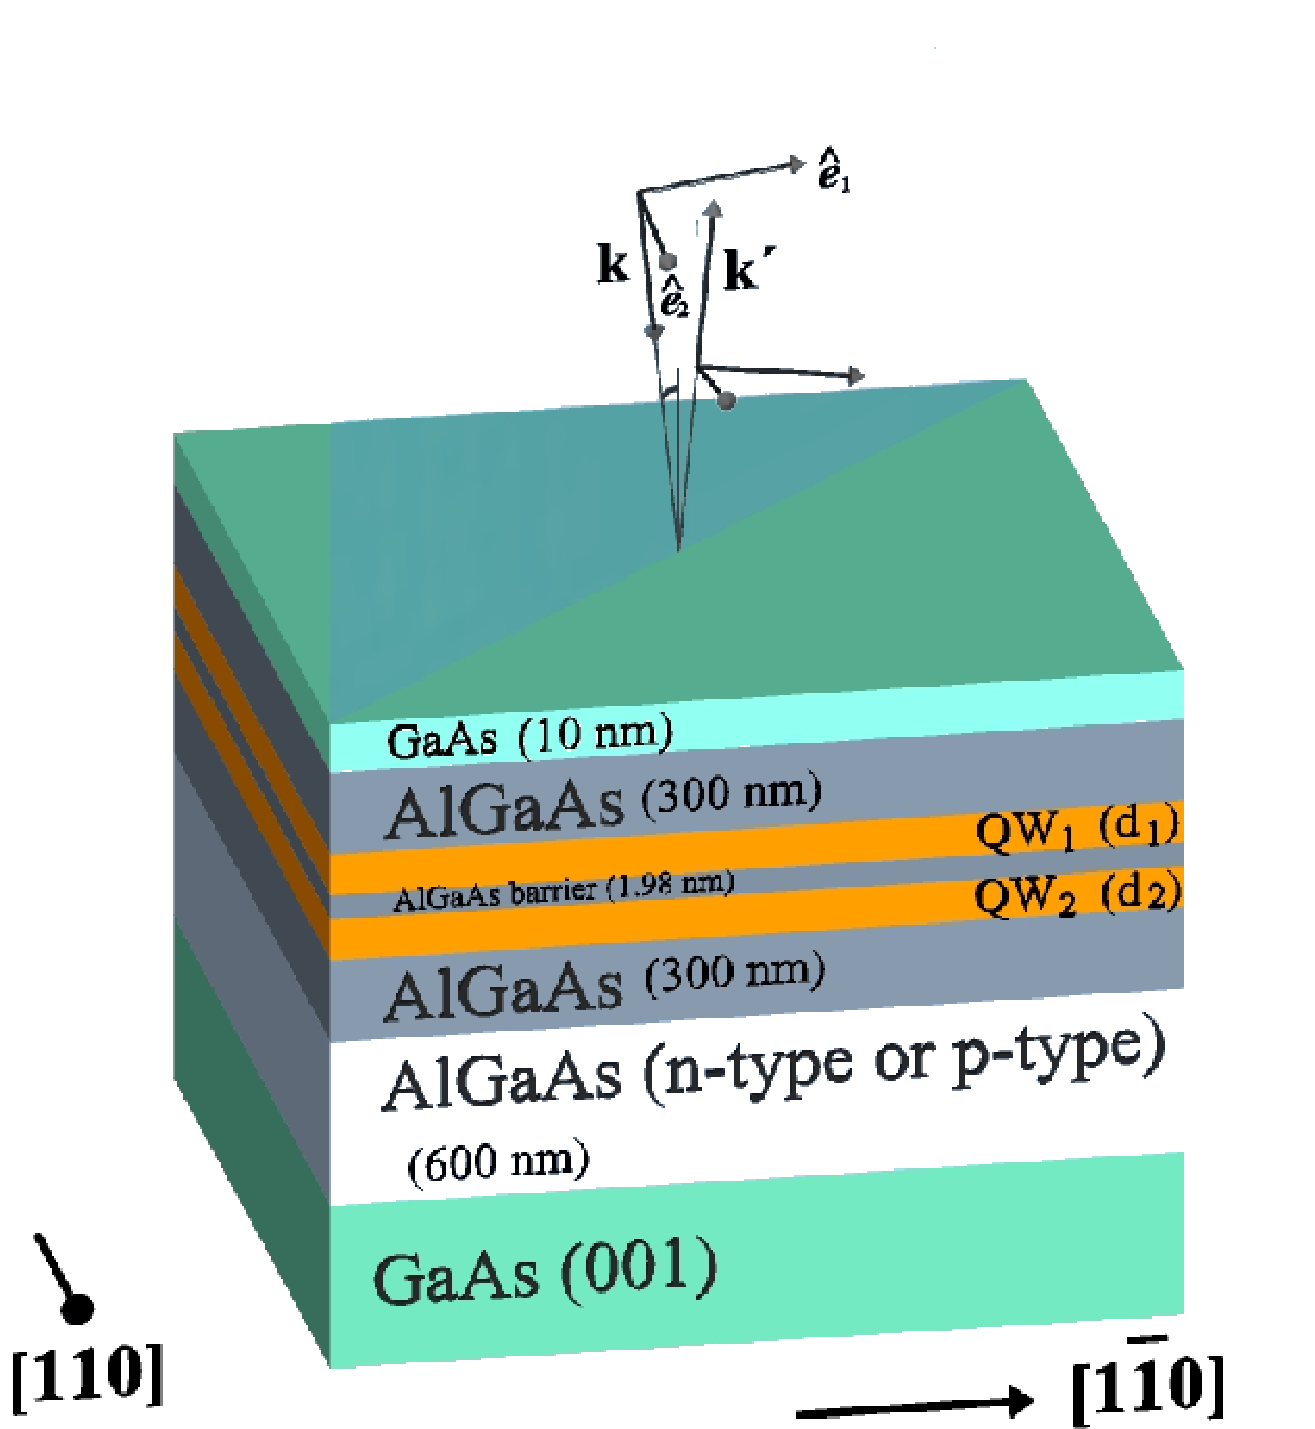
\includegraphics[width=0.3\textwidth]{../beamer-figures/results/Fig_1}};

\node<1->[anchor=north west,yshift=-3mm](i1) at (txt.south west){\includegraphics[width=0.5\textwidth,trim={0cm 0cm 0cm 2.5cm},clip]{../../figures/chapter-2/symmetry/build-ruco/sym-1-wob-beamer.pdf}};

\node<2->[anchor=north west,inner sep=0mm,yshift=-3mm](i2) at (i1.south west){\includegraphics[width=0.5\textwidth,trim={0cm 0cm 0cm 0cm},clip]{../../figures/chapter-2/symmetry/build-ruco/sym-2-wob-beamer.pdf}};


\node<2->[anchor=north west,inner sep=0mm,yshift=-5mm](i3) at (i1.north east){\animategraphics[autoplay,loop,width=0.5\textwidth,]{2}{beamer-figures/physical-model/build-ruco/aef}{0}{}};
\end{tikzpicture}
\end{frame}


\subsection{Contexto de Simetr\'ia}
\begin{frame}[t]
\frametitle{\secname}
\framesubtitle{Contexto de Simetr\'ia}
\vspace{-0.5cm}
\begin{tikzpicture}[remember picture, overlay]
\node<1->[anchor = north west, text width =0.7\textwidth, yshift = -0.75cm](txt) at (current page.north west) {
	\begin{tcolorbox}[enhanced,title =Contexto de Simetr\'ia,
	left=1mm,
	top=1mm,
	bottom=1mm,
	right=1mm,
	width =\textwidth,
	height=0.28\textheight,
	boxsep = 0cm,
	coltitle=blue,
	attach boxed title to top center={yshift=-2mm,yshifttext=-1mm},
	boxed title style={colframe=blue,
		colback=gc!90}]
	\begin{itemize}
	\item<1-> Simetr\'ia es un cambio sin cambio.
	\item<2-> Transformaciones u operaciones que no alteran un ``objeto''
	\item<3-> La Teoria de Grupos aplicada a una estructura cristalina resulta en el mapa o ruta de los electrones conocido como la Zona de Brillouin
	\end{itemize}
	\end{tcolorbox}	
};

	\node<1->[anchor=north east,xshift=-20mm,yshift=-9mm] (i1) at (current page.north east){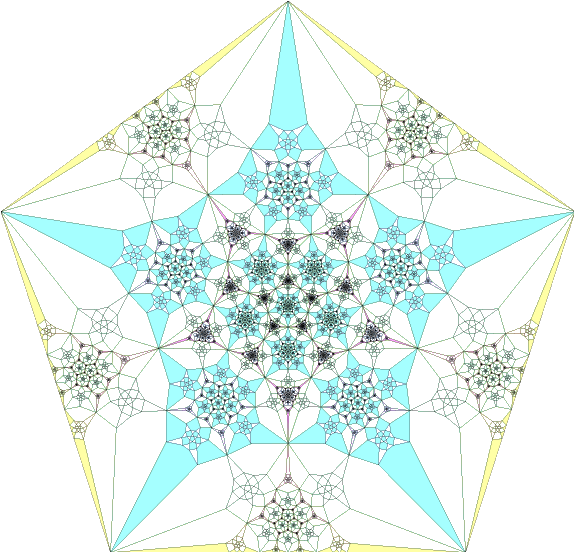
\includegraphics[width=0.33\textwidth]{../beamer-figures/physical-model/BigPlatoBig.png}};
	\def\optionc{1}

	\ifnum\optionc=1
	\node<2-3>[anchor=north west,inner sep=0mm,xshift=2mm,yshift=2mm](sym1) at (txt.south west){\animategraphics[autoplay,loop,width=0.22\textwidth,]{20}{beamer-figures/physical-model/sym1}{}{}};
	\node<2-3>[anchor=north west,inner sep=0mm,xshift=2mm](sym2) at (sym1.north east){\animategraphics[autoplay,loop,width=0.22\textwidth,]{20}{beamer-figures/physical-model/sym2}{}{}};
	\node<2-3>[anchor=north west,inner sep=0mm,xshift=2mm,yshift=-3.5mm](sym3) at (sym2.north east){\animategraphics[autoplay,loop,width=0.22\textwidth,]{20}{beamer-figures/physical-model/sym3}{}{}};
	\node<2-3>[anchor=north west,inner sep=0mm,xshift=2mm](sym4) at (sym3.north east){\animategraphics[autoplay,loop,width=0.22\textwidth,]{20}{beamer-figures/physical-model/sym4}{}{}};

	\node<2-3>[anchor=north,inner sep=0mm,xshift=0mm](sym5) at (sym1.south){\animategraphics[autoplay,loop,width=0.22\textwidth,]{20}{beamer-figures/physical-model/sym5}{}{}};
	\node<2-3>[anchor=north,inner sep=0mm,xshift=0mm](sym6) at (sym2.south){\animategraphics[autoplay,loop,width=0.22\textwidth,]{20}{beamer-figures/physical-model/sym6}{}{}};
	\node<2-3>[anchor=north,inner sep=0mm,xshift=0mm,yshift=-3mm](sym7) at (sym3.south){\animategraphics[autoplay,loop,width=0.22\textwidth,]{20}{beamer-figures/physical-model/sym7}{}{}};
	\node<2-3>[anchor=north,inner sep=0mm,xshift=0mm](sym8) at (sym4.south){\animategraphics[autoplay,loop,width=0.22\textwidth,]{20}{beamer-figures/physical-model/sym8}{}{}};

	\node<2-3>[anchor=south west, text width=\textwidth,scale=0.7,text=gc] at (current page.south west){Attribution: symotter.org/gallery};
\fi


\end{tikzpicture}
\end{frame}
	
	
\subsection{Simetr\'ia y Estructura de Bandas}
\begin{frame}[t]
\frametitle{\secname}
\framesubtitle{\subsecname}
\vspace{-0.5cm}
\begin{tikzpicture}[remember picture, overlay]
\node<1->[anchor = north west, text width =0.65\textwidth, yshift = -0.75cm](txt) at (current page.north west) {
	\begin{tcolorbox}[enhanced,title =\subsecname,
	left=1mm,
	top=1mm,
	bottom=1mm,
	right=1mm,
	width =\textwidth,
	height=0.2\textheight,
	boxsep = 0cm,
	coltitle=blue,
	attach boxed title to top center={yshift=-2mm,yshifttext=-1mm},
	boxed title style={colframe=blue,
		colback=gc!90}]
	\begin{itemize}
	\item<1-> Simetr\'ia ``Macroscopica'' +  Simetr\'ia ``Microscopica'' = Simetria del Sistema.
	\item<2-> \textcolor{red}{\emph{La s\'imetria de un sistema define las funciones base para obteener la Estructura de Bandas}}
	
	\end{itemize}
	\end{tcolorbox}	
};

\def\optionc{1}
\ifnum\optionc=1
	\node<1>[anchor=north west,inner sep=0mm,xshift=-5mm,yshift=5mm](sym1) at (txt.north east){\animategraphics[autoplay,loop,width=0.4\textwidth]{10}{beamer-figures/physical-model/sym9}{}{}};
\fi
\node<2->[anchor=north west,inner sep=0mm,xshift=0mm,yshift=-3mm] at  (txt.north east) {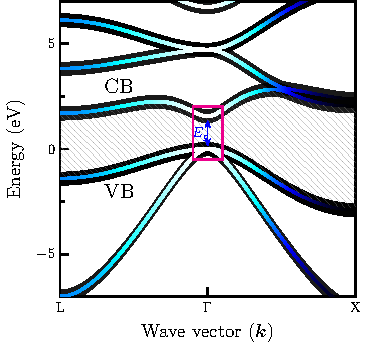
\includegraphics[width=0.35\textwidth]{../../figures/chapter-1/bands/build-ruco/bands01-beamer}};
\node<2->[anchor=south west,xshift=0mm,yshift=0mm] (i2) at (current page.south west){\includegraphics[width=\textwidth]{../../figures/chapter-2/symmetry/out/sym-0}};

\end{tikzpicture}
\end{frame}
	


\subsection{Reducci\'on de Simetria en Pozos Cu\'anticos Acoplados}
\begin{frame}[t]
\frametitle{\secname}
\framesubtitle{\subsecname}
\begin{tikzpicture}[remember picture, overlay]
\node<1->[anchor = north west, text width =0.75\textwidth, yshift = -0.75cm,scale=1](txt) at (current page.north west) {
	\begin{tcolorbox}[width=\textwidth]
	\begin{itemize}
	\item<1-> \emph{De las simetrias de un sistema se definen las propiedades del mismo.}	
	\item<2-> En 1894 Pierre Curie $\rightarrow$``principio de simetría''\\
	\emph{\color{magenta}Cuando ciertas causas producen ciertos efectos, los elementos de simetría de las causas deben encontrarse en los efectos producidos.\footnotemark[1]}
	\item<3->Ruptura de simetr\'ia en Pozos Cuanticos Acoplados
	\end{itemize}
	\end{tcolorbox}	
};

\node<1->[anchor=north west,yshift=-2mm] at (txt.north east){\includegraphics[width=0.25\textwidth]{/media/labfiles/ruco/phd-ssp/scripts/structures/GaAs1.pdf}};

\node<2>[anchor=west,yshift=-15mm](i2) at (current page.west){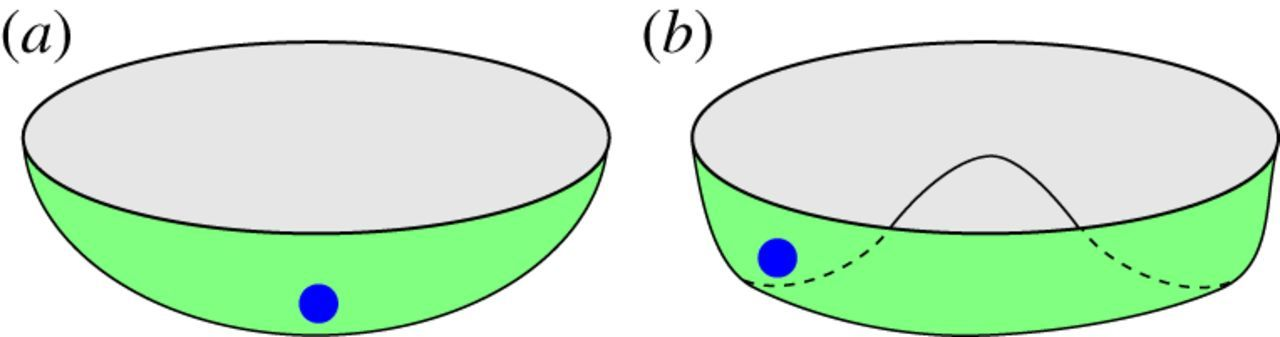
\includegraphics[width=\textwidth,trim={0cm 0cm 0cm 0cm},clip]{beamer-figures/physical-model/sym001.jpg}};
\node<2>[anchor=north west,text width=\textwidth,scale=0.8] at (i2.south west) {Kibble T. W. B. 2015Spontaneous symmetry breaking in gauge theories \textit{Phil. Trans. R. Soc. A.} \textbf{373:}20140033};
\node<2>[anchor=south west,text width=0.5\textwidth,xshift=15mm] at (i2.north west) {Unbroken symmetry};
\node<2>[anchor=south east,text width=0.5\textwidth,xshift=15mm] at (i2.north east) {Broken symmetry};

\node<3-4>[anchor=west,yshift=-15mm](i3) at (current page.west){\includegraphics[width=0.3\textwidth]{/media/labfiles/ruco/phd-ssp/scripts/structures/GaAs1.pdf}};
\node<3-4>[anchor=north,draw=white,fill=black,text=white,scale=1.25] at (i3.south) {$T_{d}$};
\node<3>[anchor=west,yshift=0mm](i4) at (i3.east){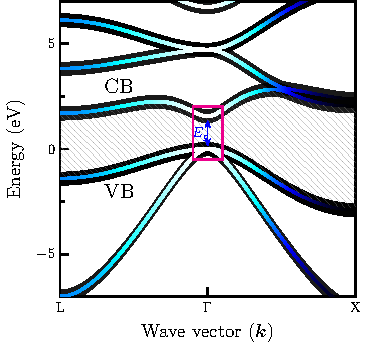
\includegraphics[width=0.4\textwidth]{../../figures/chapter-1/bands/build-ruco/bands01-beamer}};

\node<4>[anchor=north west,xshift=8mm](i5) at (i3.north east){\includegraphics[width=0.6\textwidth,trim={0cm 0cm 0cm 2.5cm},clip]{../../figures/chapter-2/symmetry/build-ruco/sym-1-wob-beamer.pdf}};
\node<4>[anchor=north,draw=white,fill=black,text=white,scale=1.25] at (i5.south) {$D_{2d}$};
\draw<4>[-{Stealth},scale=2] (i3)--(i5);

\node<5>[anchor=west,xshift=0mm,yshift=-15mm](i6) at (current page.west){\includegraphics[width=0.6\textwidth,trim={0cm 0cm 0cm 2.5cm},clip]{../../figures/chapter-2/symmetry/build-ruco/sym-1-wob-beamer.pdf}};
\node<5>[anchor=north,draw=white,fill=black,text=white,scale=1.25] at (i6.south) {$D_{2d}$};
\node<5>[anchor=west,yshift=0mm](i7) at (i6.east){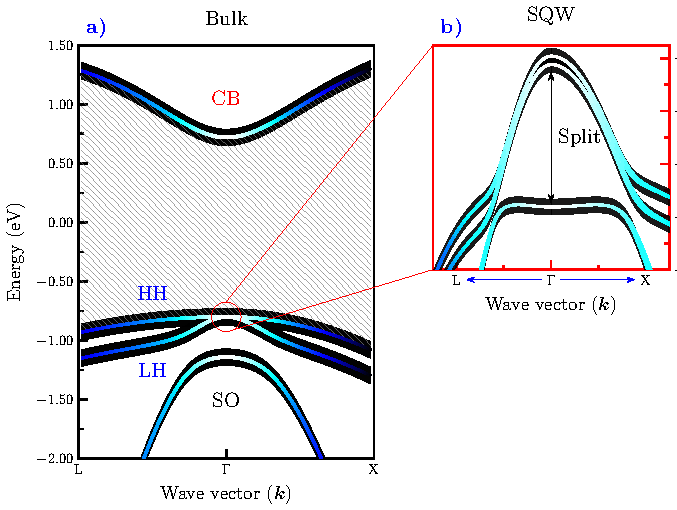
\includegraphics[width=0.6\textwidth]{../../figures/chapter-2/numerical-calculations/out/kp-bands}};

\node<6>[anchor=south,xshift=-10mm,yshift=13mm](i7) at (current page.south){\includegraphics[width=0.7\textwidth,trim={0cm 0cm 0cm 0cm},clip]{../../figures/chapter-2/symmetry/build-ruco/sym-2-wob-beamer.pdf}};
\node<6>[anchor=north,draw=white,fill=black,text=white,scale=1.25] at (i7.south) {$D_{2d}$};

\node<7>[anchor=south,xshift=-10mm,yshift=13mm](i8) at (current page.south){\includegraphics[width=0.7\textwidth,trim={0cm 0cm 0cm 0cm},clip]{../../figures/chapter-2/symmetry/build-ruco/sym-3-wob-beamer.pdf}};
\node<7>[anchor=north,draw=white,fill=black,text=white,scale=1.25] at (i8.south) {$C_{2v}$};


% ../figures/chapter-2/symmetry/out/roadmap

\end{tikzpicture}

\onslide<2->{\footnotetext[1]{Curie, P. (1894). On symmetry in physical phenomena, symmetry of an electric field and of a magnetic field. J. Phys, 3, 395-415.}}
\end{frame}
	

\begin{frame}[t]
	\frametitle{\secname}
	\framesubtitle{\subsecname}
	\begin{tikzpicture}[remember picture, overlay]
	
		\node[anchor=south west,xshift=10mm,yshift=-2mm] at (current page.south west){\includegraphics[width=0.86\textwidth,]{../../figures/chapter-2/symmetry/build-ruco/roadmap-beamer}};
	\end{tikzpicture}
\end{frame}




\subsection{Calculos Num\'ericos}
\begin{frame}[t]
\frametitle{\secname}
\framesubtitle{\subsecname}
\begin{tikzpicture}[remember picture, overlay]
\node<1->[anchor = north west, text width =0.75\textwidth, yshift = -0.75cm,scale=1](txt) at (current page.north west) {
	\begin{tcolorbox}[width=\textwidth]
	\begin{itemize}
	\item<1-> Buscando la simplicidad	
	\item<2-> La reduccion de simetria nos permite usar un modelo Uni-dimensional
	\end{itemize}
	\end{tcolorbox}	
};


\node<1>[anchor=south west,yshift=0mm](ii) at (current page.south west){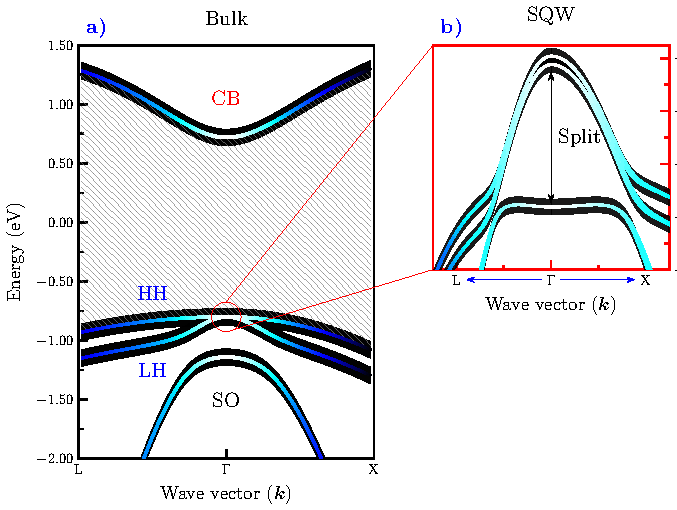
\includegraphics[width=0.9\textwidth]{../../figures/chapter-2/numerical-calculations/out/kp-bands}};

\node<1>[anchor=south east,yshift=0mm,xshift=-20mm](i2) at (current page.south east){\includegraphics[width=0.45\textwidth,trim={0cm 0cm 0cm 2.5cm},clip]{../../figures/chapter-2/symmetry/build-ruco/sym-1-wob-beamer.pdf}};


\node<2>[anchor=south west,yshift=-2mm](i3) at (current page.south west){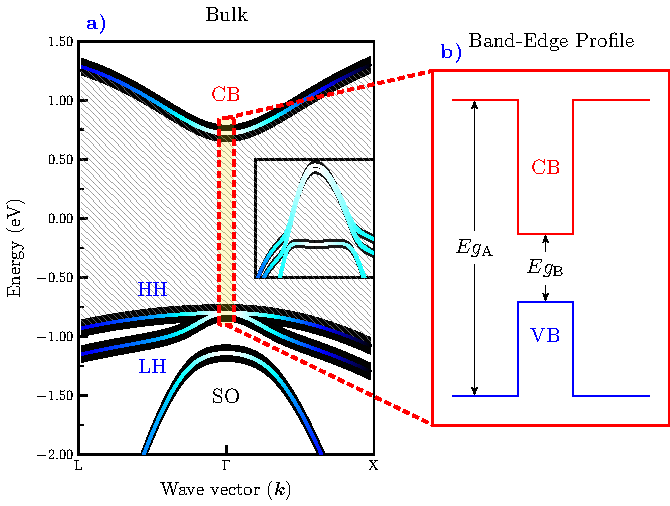
\includegraphics[width=0.85\textwidth]{../../figures/chapter-2/numerical-calculations/out/band-edge}};
\node<3->[anchor=south west,inner sep=0mm](i3) at (current page.south west){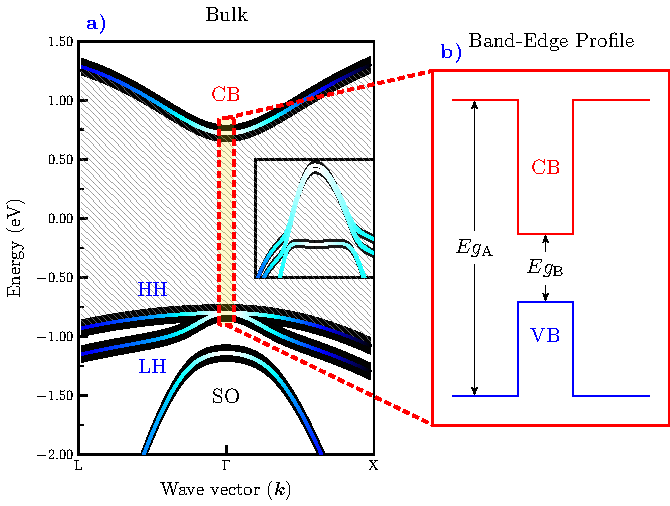
\includegraphics[width=0.4\textwidth]{../../figures/chapter-2/numerical-calculations/out/band-edge}};

\node<3->[anchor=north west,text width=0.5\textwidth](e1) at (txt.south west){
\begin{align}
	\textbf{H}\psi(z)&=E\psi(z)\\
	H_{z} &= \dfrac{p_{z}^{2}}{2m^{*}(z)}+V(z)
\end{align}
};

\node<4->[anchor=north west,text width=0.5\textwidth](e2) at (e1.south west){
	\begin{equation}
		\begin{split}
		\left[-\dfrac{\hbar^2}{2m_{jz}^{*}}\dfrac{d^2}{dz^2}+V(z) \right]\psi_{nj}(z)&= E_{nj}\psi_{nj}(z),\\
																	   j&=e,\mathrm{hh},\mathrm{lh}.
		\end{split}
	\end{equation}
};


\node<4->[anchor=north west,yshift=0mm](i3) at (e1.north east){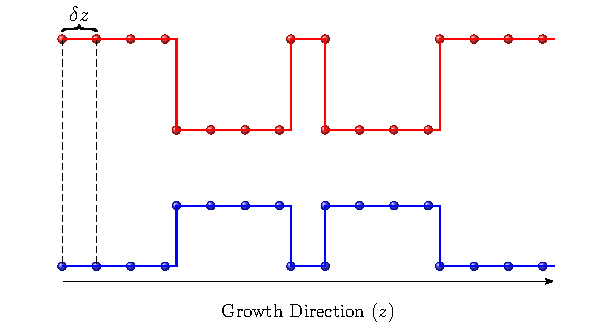
\includegraphics[width=0.53\textwidth]{../../figures/chapter-2/numerical-calculations/out/fdm-potential-1}};
\node<5->[anchor=north west,text width=0.7\textwidth,xshift=-13mm,yshift=-3mm,scale=0.9](e3) at (i3.south west){\begin{equation*}
	-\dfrac{\hbar}{2m^{*}}\left[\dfrac{\psi(z+\delta z)-2\psi(z)+\psi(z-\delta z)}{(\delta z)^2}\right] + V(z)\psi(z)=E\psi(z).
\end{equation*}};
\node<5->[anchor=north west,text width=0.7\textwidth,xshift=0mm,yshift=0mm,scale=1](e4) at (e3.south west){
	\begin{equation*}
		a_{i}\psi_{i-1}+b_{i}\psi_{i}+c_{i}\psi_{i+1}=E\psi_{i}
	\end{equation*}
};

\node<5>[anchor=north west,text width=0.7\textwidth,xshift=1mm,yshift=0mm,scale=0.8](e5) at (e4.south west){
\begin{equation*}
	a_{i+1}=c_{i}= -\dfrac{\hbar^2}{2m^{*}_{i+\frac{1}{2}}(\delta z)^2} \quad \text{and}\quad b_{i}=\dfrac{\hbar^{2}}{2(\delta z)^2}\left(\dfrac{1}{m^{*}_{i+\frac{1}{2}}}+\dfrac{1}{m^{*}_{i-\frac{1}{2}}}\right)+V_{i}.
\end{equation*}
};
\node<6->[anchor=north west,text width=0.7\textwidth,xshift=0mm,yshift=0mm,scale=0.8](e5) at (e4.south west){
	\begin{equation*}
		\textbf{H}=\begin{pmatrix}
			b_{1} & c_{1} & 0      &\cdots & 0\\
			a_{2} & b_{2} & c_{2}  &\cdots &0\\
			0     &\ddots &\ddots  &\ddots&0\\
			\vdots&\cdots &a_{N-1} &b_{N-1}&c_{N-1}\\
			0     &\cdots&0        &a_{N}  &b_{N} 
		\end{pmatrix}
	\end{equation*}
};

\end{tikzpicture}

\end{frame}


\begin{frame}[t]
	\frametitle{\secname}
	\framesubtitle{\subsecname}
	\begin{tikzpicture}[remember picture, overlay]
	\node<1->[anchor = north west, text width =0.7\textwidth, yshift = -0.75cm,scale=1](txt) at (current page.north west) {
		\begin{tcolorbox}[width=\textwidth]
		\begin{itemize}
		\item<1-> Resultados num\'ericos
		\end{itemize}
		\end{tcolorbox}	
	};
	
	\node<1>[anchor=north west,text width=0.7\textwidth](e2) at (txt.south west){
		\begin{equation}
			V(z),m^{*}(z)=\begin{cases}
				\text{\algaasx{0.2}}\quad &0<z<20\text{ nm}\\
				\text{GaAs}\quad    &20<z<26\text{ nm}\\
				\text{\algaasx{0.2}}\quad &26<z<32\text{ nm}\\
				\text{GaAs}\quad    &32<z<38\text{ nm}\\
				\text{\algaasx{0.2}}\quad &38<z<58\text{ nm},
			\end{cases}
		\end{equation}
};

\node<1>[anchor=south west,inner sep=0mm,yshift=5mm](i3) at (current page.south west){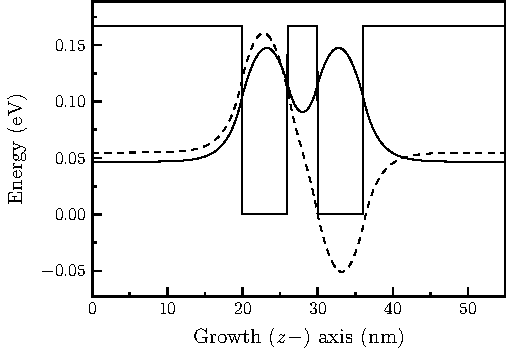
\includegraphics[width=\textwidth]{../../figures/chapter-2/numerical-calculations/out/harrison-wells}};
\node<2->[anchor=south west,inner sep=0mm,xshift=10mm](i3) at (current page.south west){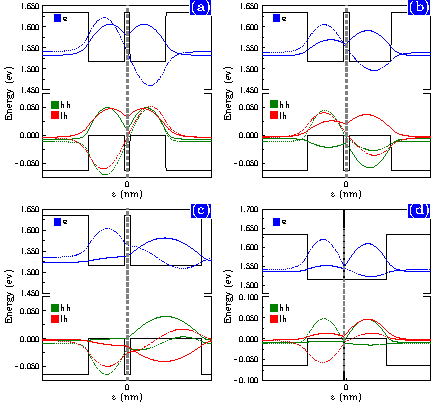
\includegraphics[width=0.8\textwidth]{../../figures/chapter-2/numerical-calculations/build-ruco/numerical-results}};
	\end{tikzpicture}
	
	\end{frame}